\documentclass[12pt]{article}

\usepackage{fullpage} % Package to use full page
\usepackage{parskip} % Package to tweak paragraph skipping
\usepackage{tikz} % Package for drawing
\usepackage{amsmath}
\usepackage{hyperref}
\usepackage{minted}
\usepackage{pythonhighlight}
\usepackage{cite}
\usepackage{bm}
\usepackage[style=apa, backend=biber]{biblatex}
\addbibresource{references.bib} 
\usepackage{caption}


\title{MA4270 Project: Comparative Analysis of GBDT and XGBoost in Classification Challenges}
\author{
    HUANG RUI\\
    \textit{A0275006L}
    \and
    LIN YI-HSUAN\\
    \textit{A0275070J}
}

\date{\today}

\begin{document}

\maketitle

\section{About this Project}
The aim of this project is to explore the effectiveness and optimization of XGBoost compared to the traditional Gradient Boosted Decision Tree (GBDT) model in classification problems. \\

In this project we will perform the following parts in sequence: acquiring data and data preprocessing, training the model, and evaluating the model. By using both GBDT and XGBoost models on the same dataset, this project attempts to carefully compare and analyze the performance metrics such as accuracy, precision, recall, and F1 scores in order to highlight the advantages of XGBoost in handling the classification task. \\

Through the comparative analysis, we aim to provide a comprehensive overview of how XGBoost improves upon the GBDT framework to gain insights into its applicability and superiority in solving classification challenges.\\

\section{Introduction to the Dataset and Prepocessing}
This dataset contains meteorological observation data from various locations on different dates. It covers multiple meteorological indicators such as temperature, rainfall, evaporation, and sunshine hours, making it suitable for climate research, weather forecasting, or supporting the training and validation of machine learning models.

\subsection{Detailed Information of the Dataset}


The dataset includes the following key features:
\begin{itemize}
    \item \textbf{Date}: The date of observation.
    \item \textbf{Location}: The location of the meteorological observation.
    \item \textbf{MinTemp} and \textbf{MaxTemp}: The minimum and maximum temperature of the day.
    \item \textbf{Rainfall}: The amount of rainfall (in millimeters) for the day.
    \item \textbf{Evaporation}: The amount of evaporation (in millimeters) for the day.
    \item \textbf{Sunshine}: The number of sunshine hours for the day.
    \item \textbf{WindGustDir} and \textbf{WindGustSpeed}: The direction and speed of the maximum wind gust.
    \item \textbf{WindDir9am} and \textbf{WindDir3pm}: The wind direction at 9 AM and 3 PM.
    \item \textbf{Humidity9am} and \textbf{Humidity3pm}: The humidity percentage at 9 AM and 3 PM.
    \item \textbf{Pressure9am} and \textbf{Pressure3pm}: The atmospheric pressure (in hPa) at 9 AM and 3 PM.
    \item \textbf{Cloud9am} and \textbf{Cloud3pm}: The cloud cover (in oktas) at 9 AM and 3 PM.
    \item \textbf{Temp9am} and \textbf{Temp3pm}: The temperature at 9 AM and 3 PM.
    \item \textbf{RainToday} and \textbf{RainTomorrow}: Indicators of rain for the current and next day (Yes/No).
\end{itemize}

\subsection{Data Visualization}
\subsubsection*{Scatter Plot Visualization of Features and Label}
Using the \texttt{sns.pairplot} function, we selected three features: \textit{Rainfall} (amount of rainfall), \textit{Evaporation} (amount of evaporation), and \textit{Sunshine} (amount of sunshine), along with the target variable \textit{RainTomorrow} (whether it will rain tomorrow or not) for the creation of scatter plot visualizations. This allows us to intuitively observe the general distribution of whether it will rain tomorrow (\textit{Yes} or \textit{No}) under different feature values.


\subsubsection*{Bar Plot Visualization Based on Categorical Features}
Firstly, we filtered out all categorical features except for the target variable \textit{RainTomorrow}. Then, for each categorical feature, we calculated the count of values labeled as "Yes" and "No". Taking \textit{Location} as an example, we utilized the \texttt{sns.barplot} function to draw two bar plots. These plots respectively show the distribution of the number of occurrences for rain (\textit{Yes}) and no rain (\textit{No}) tomorrow at different locations, thereby revealing the potential impact of different locations on rain prediction.
\subsubsection*{Heatmap Visualization of Correlation Between Features and RainTomorrow}
To elucidate the linear relationships and dependencies between the numerical features and the target variable `RainTomorrow`, we computed a correlation matrix. This matrix was then visualized using a heatmap, facilitated by the \texttt{sns.heatmap} function from the seaborn library. The heatmap employs a color-coded scheme where the intensity of the color and the annotations within each cell indicate the magnitude of correlation between the variables. This visualization method is instrumental in pinpointing features that exhibit a strong linear relationship with the target variable, `RainTomorrow`, thereby highlighting those that might significantly influence the prediction of rain on the following day. The gradient from warm to cool colors corresponds to the transition from positive to negative correlation values.
\subsubsection*{Cumulative Distribution Function (CDF) Visualization of Rainfall by RainTomorrow}
Building upon our investigation into feature correlations, we delved into understanding the impact of the `Rainfall` feature on predicting rain the next day (`RainTomorrow`). By segregating the dataset into instances classified as `Yes` (rain) and `No` (no rain) for `RainTomorrow`, we calculated and visualized the Cumulative Distribution Function (CDF) for each subset. This process entailed sorting the `Rainfall` data in ascending order and plotting it against its cumulative percentage. The CDF plots for instances when `RainTomorrow` equals `Yes` and `No` offer a vivid illustration of how the likelihood of rain the subsequent day escalates with the quantity of rainfall. 


\begin{figure}[htbp]
  \centering
  \begin{minipage}[b]{0.49\textwidth}
    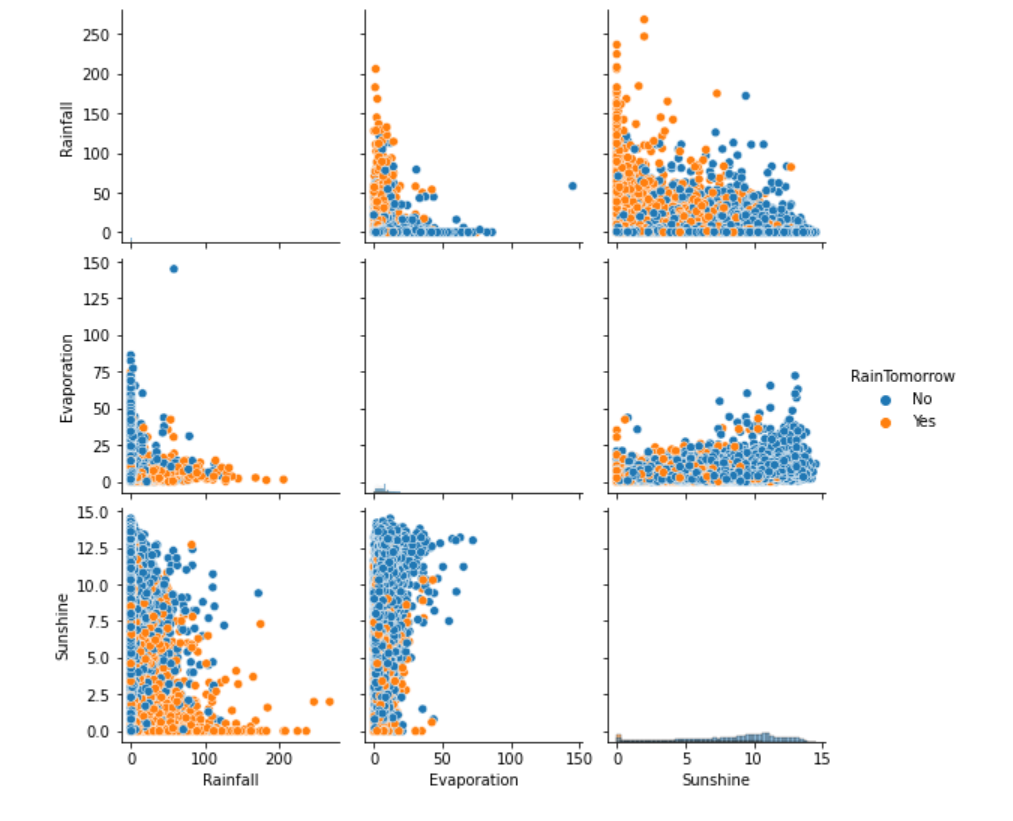
\includegraphics[width=\textwidth]{1.png}
    % \label{fig:figure3}
  \end{minipage}
  \hfill
  \begin{minipage}[b]{0.49\textwidth}
    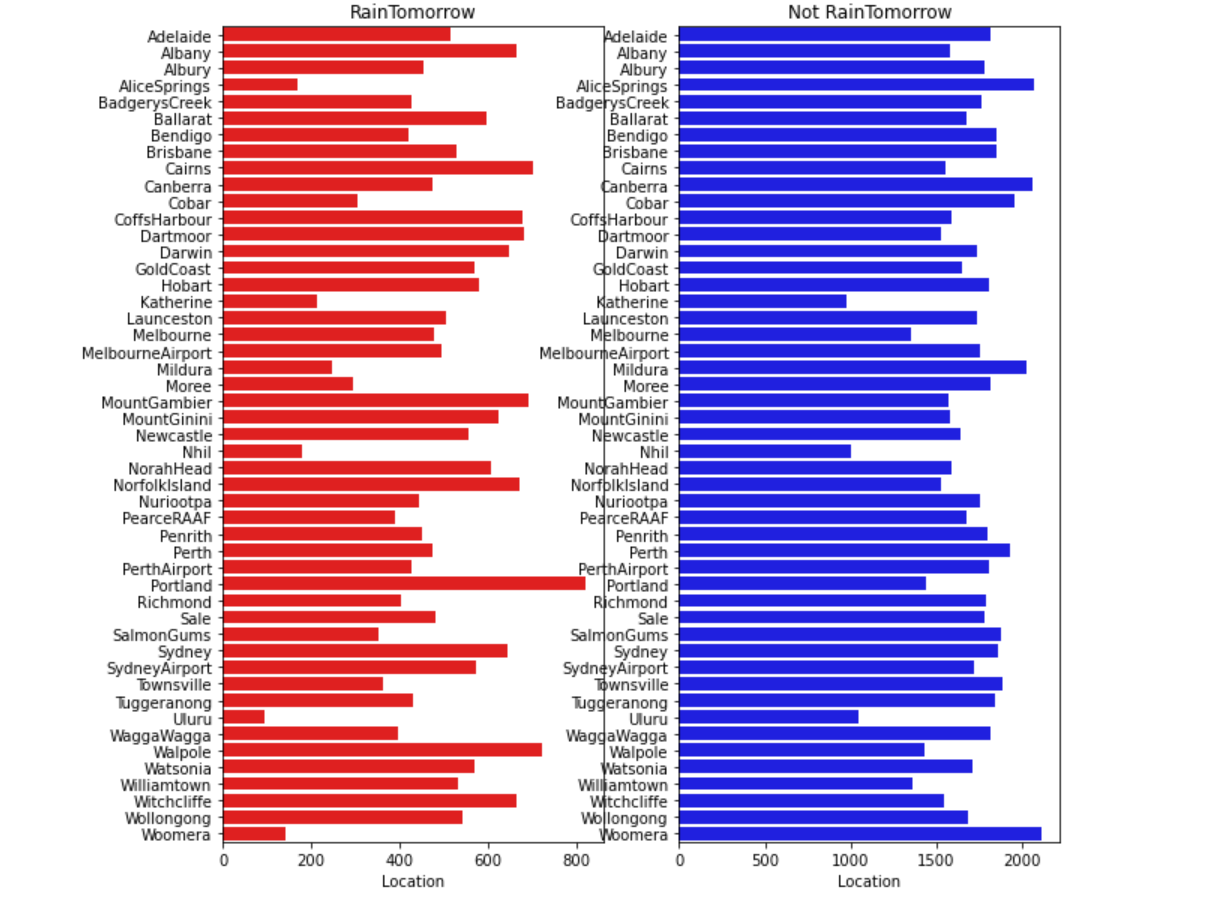
\includegraphics[width=\textwidth]{2.png}
    % \label{fig:figure4}
  \end{minipage}
\end{figure}
\begin{figure}[htbp]
  \centering
  \begin{minipage}[b]{0.49\textwidth}
    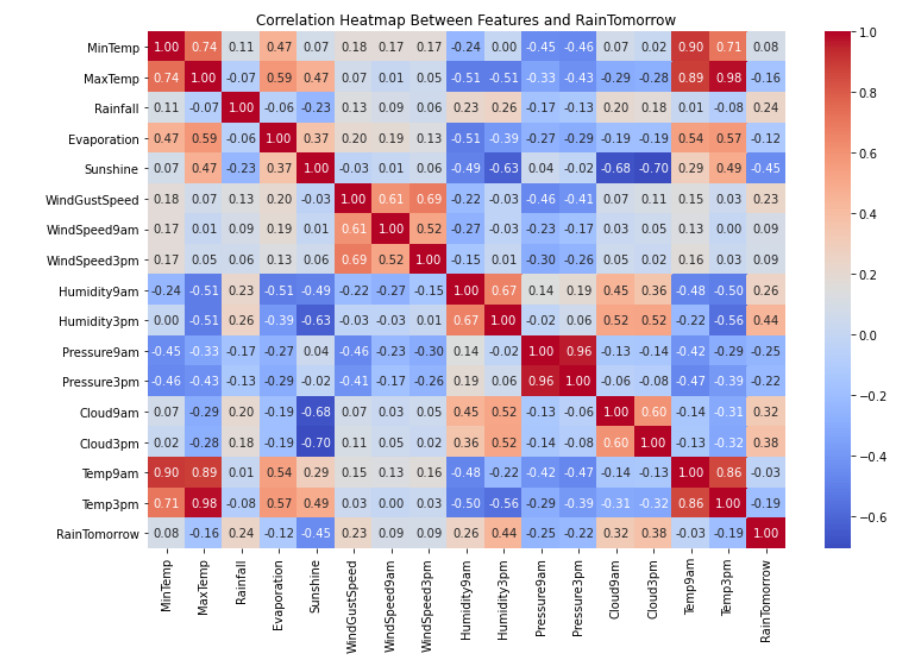
\includegraphics[width=\textwidth]{3.png}
    % \label{fig:figure3}
  \end{minipage}
  \hfill
  \begin{minipage}[b]{0.49\textwidth}
    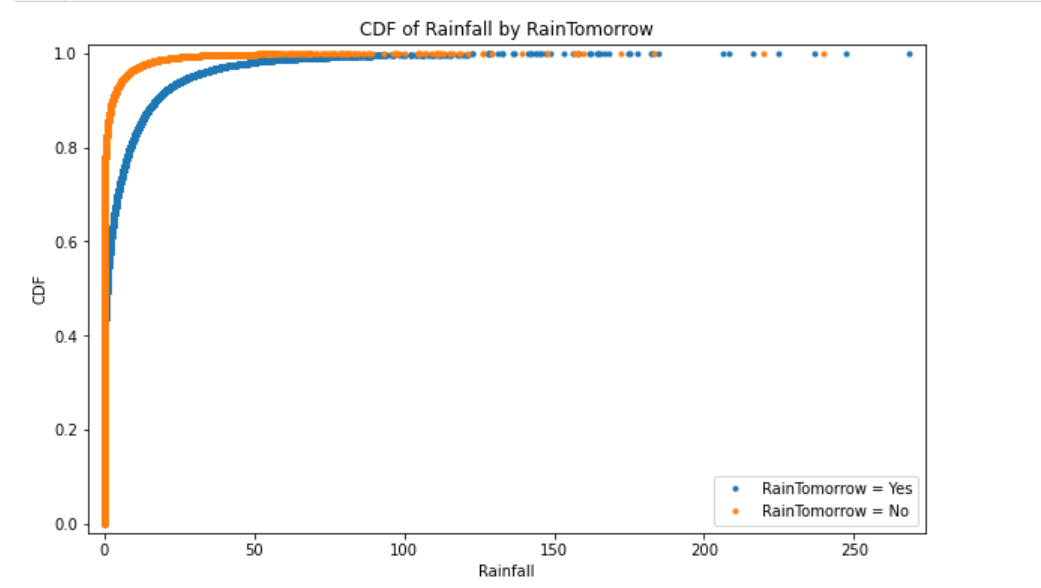
\includegraphics[width=\textwidth]{4.png}
    % \label{fig:figure4}
  \end{minipage}
\end{figure}

Through these visualizations, we are able to gain a clearer understanding of the patterns and trends within the data, providing an intuitive foundation for subsequent model training and analysis.
\subsection{Data Preprocessing}
\subsubsection*{library usage}
During the data preprocessing process, we utilized several key Python libraries for execution. Initially, the \texttt{requests} library was employed to download the dataset from the internet. Subsequently, the \texttt{pandas} library was used for reading and conducting preliminary processing of the data, offering significant convenience in data analysis and handling. To directly read CSV from the downloaded text data, we also used \texttt{StringIO}, which allows us to treat strings as if they were files.

In the data preprocessing phase, Scikit-learn (\texttt{sklearn}) provided an array of tools and methods for imputing missing values, standardizing features, and encoding. We integrated the processing steps for numerical and categorical features through \texttt{ColumnTransformer} and \texttt{Pipeline}, making the preprocessing procedure both efficient and manageable. Finally, \texttt{train\_test\_split} assisted in dividing the processed data into training and testing sets, preparing for model training and evaluation.

\begin{minted}{python}
import requests
import pandas as pd
from io import StringIO
from sklearn.model_selection import train_test_split
from sklearn.preprocessing import LabelEncoder, StandardScaler, OneHotEncoder
from sklearn.compose import ColumnTransformer
from sklearn.impute import SimpleImputer
from sklearn.pipeline import Pipeline
\end{minted}
\subsubsection*{data preprocessing methods}
% We use the \texttt{requests} library to download the dataset from the specified URL, and by utilizing the \texttt{pandas} library and \texttt{StringIO} object, we are able to directly read the CSV format dataset from the obtained text data, without the need to first save the data to the local disk.

% For numerical features, we fill all missing values with $-1$, thereby maintaining the integrity of the data while also providing a clear marker for missing situations.

% Considering that most machine learning algorithms require numerical input, we apply label encoding to categorical features, aiming to convert text labels into integer labels that are easier for the model to understand.

When processing the data, several key steps were taken to ensure the quality and suitability of the data. Firstly, the method of filling missing values with the median was employed to handle numerical features, which helps maintain data integrity and avoid adverse effects on the model. 

Subsequently, for categorical features, missing values were filled, and then converted into one-hot encoding format. Additionally, standardization was applied to numerical features to ensure that they have similar scales, thus avoiding issues caused by differences in feature scales. Finally, the ColumnTransformer was utilized to combine these data processing steps and apply them to the entire dataset, ensuring a consistent data processing workflow.

\begin{minted}{python}

\end{minted}
% \section{Usage Instructions}
% This dataset is suitable for fields such as meteorological research and weather prediction model training. The data is stored in CSV format and can be read with the following code snippet:

% \begin{verbatim}
%     import pandas as pd
%     data = pd.read_csv("path_to_dataset/train1.csv")
% \end{verbatim}

\section{GBDT}
\subsection{Introduction to GBDT}
GBDT or Gradient Boosting Decision Trees, is a popular machine learning algorithm, or boosting algorithms or we can say it is an ensemble model that combines multiple weak learners (decision trees) to create a strong learner and make more accurate predictions.\\

In GBDT, we actually train multiple decision trees, but each subsequent tree is trained to correct the errors made by the previous trees. Specifically, after training the first decision tree, we calculate the residuals(the errors made by the first tree) between the predicted values and the actual values. We then use these residuals as the target variable for training the second decision tree. The second decision tree is then trained on the residuals, and it tries to predict the remaining errors in the target variable that were not captured by the first tree. Now, the predictions from the second tree are then added to the predictions of the first tree, creating a new set of predictions. We then repeat this process by training a third decision tree on the residuals from the second tree, a fourth tree on the residuals from the third tree, and so on, until we have a set of trees that can accurately predict the target variable.\\

Each decision tree in GBDT is a weak learner, meaning that it is not particularly good at making accurate predictions on its own. However, if we combine many weak learners (i.e. each decision tree ) it can achieve strong predictive performance or We can say that it works by iteratively adding decision trees to an ensemble, with each tree trying to correct the errors made by the previous trees means each tree is not trained from scratch. Instead, the subsequent trees are trained to improve upon the predictions of the previous trees. Specifically, it first trains a decision tree on the dataset and calculates the error between the predicted and actual values. Then, it trains a new decision tree on the residual errors from the previous tree, and adds this new tree to the ensemble.\\

\subsection{The Algorithm of GBDT}
\subsubsection*{ALGORITHM  (Gradient Boosting Decision Trees)}

\begin{enumerate}
    \item \( F_0(\mathbf{x}) = \arg\min_\rho \sum_{i=1}^{N} L(y_i, \rho) \)
    \item For \( m = 1 \) to \( M \) do:
    \item \( \hat{y}_i = -\left[ \frac{\partial L(y_i, F(\mathbf{x}_i))}{\partial F(\mathbf{x}_i)} \right]_{F(\mathbf{x})=F_{m-1}(\mathbf{x})} \), for \( i = 1, \ldots, N \)
    \item \( a_m = \arg\min_{a, \beta} \sum_{i=1}^{N}[\hat{y}_i - \beta h(\mathbf{x}_i; a)]^2 \)
    \item \( \rho_m = \arg\min_{\rho} \sum_{i=1}^{N} L(y_i, F_{m-1}(\mathbf{x}_i) + \rho h(\mathbf{x}_i; a_m)) \)
    \item \( F_m(\mathbf{x}) = F_{m-1}(\mathbf{x}) + \rho_m h(\mathbf{x}; a_m) \)
    \item \(endFor\\
    end \; Algorithm\)
\end{enumerate}

\subsection{Implement of GBDT}
After knowing about the algorithm of GBDT, let's apply it in the preprocessed dataset. We first use the training set to train the machine learning model. After that, we test it in the training and test sets to detect the situation of overfitting. Here are the codes:
\begin{minted}{python}
from sklearn.ensemble import GradientBoostingClassifier
clf = GradientBoostingClassifier(n_estimators=100, learning_rate=1.0, 
        max_depth=1, random_state=0)
clf = clf.fit(X_train, y_train)
predictions_train = clf.predict(X_train)
predictions_test = clf.predict(X_test)
\end{minted}
There are many hyper-parameters used in the function of \textit{GradientBoostingClassifier} to improve the performance of this model.\\
We will select some of them that tuned commonly to introduce:\\
\begin{itemize}
    \item \texttt{{learning{\_{\,rate}}}:float,default=0.1}: Learning rate shrinks the contribution of each tree by learning{\_{\,rate}}. There is a trade-off between learning{\_{\,rate}} and n\_{\,estimators}.
    \item \texttt{n\_\,estimators:int,default=100}: The number of boosting stages to perform. Gradient boosting is fairly robust to over-fitting so a large number usually results in better performance.
    \item \texttt{max\_\,depth:int or None,default=3}: Maximum depth of the individual regression estimators. The maximum depth limits the number of nodes in the tree. Tune this parameter for best performance; the best value depends on the interaction of the input variables. If None, then nodes are expanded until all leaves are pure or until all leaves contain less than min\_\,samples\_\,split samples.
    \item \texttt{random\_\,state:int,RandomState instance or None,default=None}: Controls the random seed given to each Tree estimator at each boosting iteration. In addition, it controls the random permutation of the features at each split. It also controls the random splitting of the training data to obtain a validation set if n\_\,iter\_\,no\_\,change is not None. Pass an int for reproducible output across multiple function calls.
\end{itemize}
\subsection{Evaluation of GBDT}
We use four target functions to evaluate the performance of GBDT: Accuracy, Precision, Recall and F1 score. We will explain them one after another later. Here are the codes:
\begin{minted}{python}
# accuracy
accuracy_train = accuracy_score(y_train, predictions_train)
accuracy_test = accuracy_score(y_test, predictions_test)

# precision
precision_train = precision_score(y_train, predictions_train, average='binary')
precision_test = precision_score(y_test, predictions_test, average='binary')

# recall
recall_train = recall_score(y_train, predictions_train, average='binary')
recall_test = recall_score(y_test, predictions_test, average='binary')

# F1 score
f1_train = f1_score(y_train, predictions_train, average='binary')
f1_test = f1_score(y_test, predictions_test, average='binary')
\end{minted}
For accuracy:\\
If $\hat{y}_i$ is the predicted value of the $i$-th sample and $y_i$ is the corresponding true value, then the fraction of correct predictions over $n_{\text{samples}}$ is defined as
\[
\text{accuracy}(y, \hat{y}) = \frac{1}{n_{\text{samples}}} \sum_{i=0}^{n_{\text{samples}}-1} 1(\hat{y}_i = y_i)
\]
where $1(x)$ is the indicator function.\\
For precision, recall and F1 score:\\
We first introduce the confusion matrix. By definition, entry $i,j$ in a confusion matrix is the number of observations actually in group $i$, but predicted to be in group $j$. \\
In a binary classification task, the terms 'positive' and 'negative' refer to the classifier’s prediction, and the terms 'true' and 'false' refer to whether that prediction corresponds to the external judgment (sometimes known as the 'observation'). Given these definitions, we can formulate the following table:
\begin{table}[h]
\centering
\begin{tabular}{|c|c|}
\hline
\textbf{tp (true positive)} & \textbf{fp (false positive)} \\
Correct result & Unexpected result \\
\hline
\textbf{fn (false negative)} & \textbf{tn (true negative)} \\
Missing result & Correct absence of result \\
\hline
\end{tabular}
\caption*{Confusion Matrix}
\end{table}
Therefore, we can define the notions of precision and recall:
\[
\text{precision} = \frac{tp}{tp + fp},
\]

\[
\text{recall} = \frac{tp}{tp + fn},
\]


F-measure is the weighted harmonic mean of precision and recall, with precision’s contribution to the mean weighted by some parameter $\beta$:
\[
F_{\beta} = (1 + \beta^2) \cdot \frac{\text{precision} \times \text{recall}}{\beta^2 \cdot \text{precision} + \text{recall}}
\]
When $\beta = 1$, we get the F1 score:
\[
F_1 = 2 \times \frac{\text{precision} \times \text{recall}}{\text{precision} + \text{recall}}
\]


\section{XGBoost}

XGBoost was developed in 2016 by Professor Tianqi Chen from the University of Washington as an extensible machine learning system. It is a powerful software package designed to solve classification, regression, or ranking problems. XGBoost includes Gradient Boosting Decision Tree (GBDT) models and has significantly optimized the algorithms within, ensuring not only high precision but also extremely fast computational speed. For a period, it became an important tool in the fields of data mining and machine learning, both domestically and internationally.

Considerable effort has been put into system optimization and delving into the principles of machine learning with XGBoost. Its scalability, portability, and accuracy have greatly pushed the boundaries of machine learning computation, allowing XGBoost to run more than ten times faster than the popular solutions at the time on a single machine, and even capable of handling up to billions of data points in distributed systems.

XGBoost has also been widely applied in solving various problems in both the industrial and academic sectors, such as forecasting retail sales, classifying high-energy physics events, categorizing web text; predicting user behavior, detecting motion, estimating advertisement click-through rates, classifying malware, forecasting disaster risks, and predicting dropout rates in online courses. While domain-specific data analysis and feature engineering also play crucial roles in these solutions, the widespread choice of XGBoost by learners and practitioners highlights the package's importance and impact.



\subsection{Introduction to the Principle}

XGBoost enhances the GBDT model and overcomes several limitations of the traditional GBDT:
\begin{enumerate}
    \item Traditional GBDT can only handle the second-order loss function, but XGBoost can also handle the first-order loss function.
    \item Added a regularization term to the traditional CART tree generation criteria, which helps to prevent overfitting.
    \item Added a missing value handling strategy.
    \item Increased the robustness of the model by adding random features.
\end{enumerate}

XGBoost has a unique handling strategy for the missing values of features, which greatly improves the usability of the model for various datasets. Suppose a feature has a non-missing rate of 70\%, we would generally think that 3000 samples out of a total of 3000 would have non-missing values for this feature. But in reality, out of 4000 samples, there may be only 2600 non-missing values, and among the 3500 samples that follow, there may be another 50 samples with missing values, adding complexity to the model... In essence, the handling strategy for missing values in XGBoost has greatly reduced the difficulty of preprocessing the data!

The basic principles of XGBoost for building a CART tree are as follows: (1) For CART trees, construct as usual. (2) For missing values, assign them a default direction.

XGBoost constructs a new tree through the following function, where \( f_t(x) \) is the new function of the tree, and \( h_t(x) \) is the function of the new branch, formalized as follows:

\[
f_t(x) = \sum_{t=1}^{T} h_t(x)
\]

The updated model in each iteration adds a new tree to the last iteration of the model, formalized as:

\[
f_t(x) = f_{t-1}(x) + h_t(x)
\]

The objective function of the model in the \( t \)-th iteration is formalized as:

\[
r_{t,i} = y_i - f_{m-1}(x_i)
\]

Each iteration essentially solves for a new \( h_t \), and the CART tree is built based on \( -1(x_i) \) from the previous iteration.


\subsection*{Implement of XGBoost}
During the model training phase, we chose to use the XGBoost algorithm by instantiating the \texttt{XGBClassifier} class. We created an instance of the XGBoost model and configured several key hyperparameters:

\begin{itemize}
    \item \texttt{use\_label\_encoder=False}: Specifies not to use the built-in label encoder, following the updated recommendations for XGBoost, suitable for labels that have been preprocessed.
    \item \texttt{eval\_\,metric='logloss'}: Sets the model evaluation metric to logloss, which measures the discrepancy between the model's probability predictions and the actual labels. The smaller the logloss, the more accurate the model's predictions.
    \item \texttt{n\_estimators=200}: Sets the number of trees to build to 200, directly impacting the model's complexity and learning capabilities.
    \item \texttt{max\_depth=8}: Controls the maximum depth of each tree, affecting the model's learning details and computational burden.
    \item \texttt{learning\_{\,rate}=0.1}: Sets the learning rate, determining the contribution of each tree to the final prediction. A lower learning rate benefits model generalization .
\end{itemize}
\subsection*{Visualization Analysis of Feature Importance}
This code generates a bar chart visualizing the importance of features within an XGBoost model. In this visualization:
\begin{figure}[htbp]
  \centering
  \begin{minipage}[b]{0.75\textwidth}
    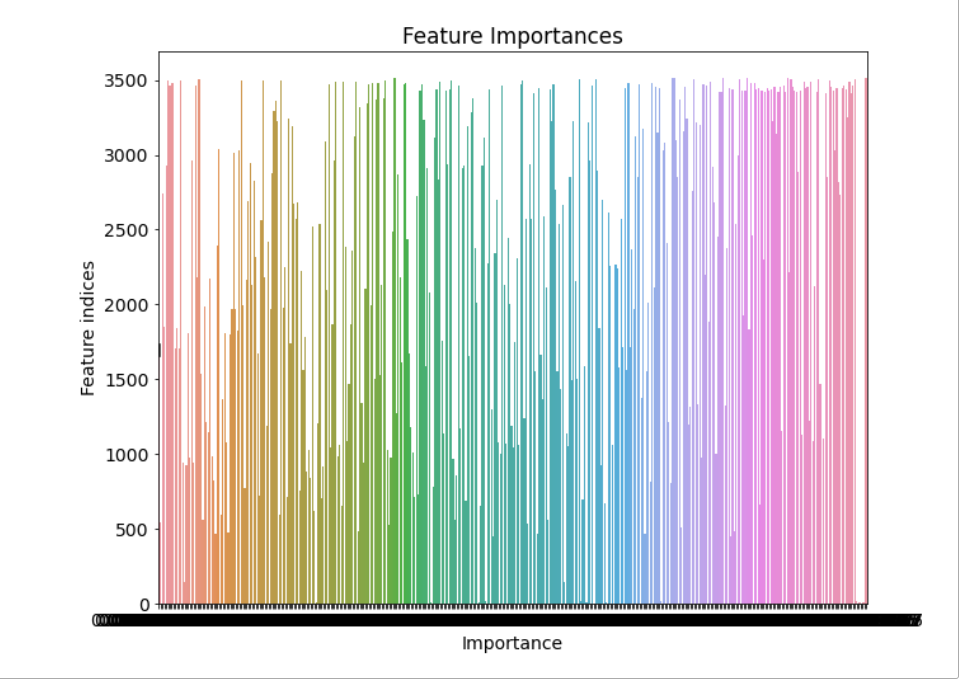
\includegraphics[width=\textwidth]{5.png}
    % \label{fig:figure3}
  \end{minipage}
  \end{figure}
\begin{itemize}
    \item The \textbf{Y-axis} lists the features of the model, typically represented by indices, with each feature corresponding to a bar.
    \item The \textbf{X-axis} represents the importance of each feature, usually a numerical value indicating the contribution of the feature to the prediction outcome during the model training process.
    \item The length of each bar signifies the importance of the feature; longer bars indicate that the feature is more significant in the model's decision-making process.
\end{itemize}

This chart provides a straightforward way to see which features have the most significant impact on the model's predictions, thereby offering insights into how the model makes its decisions. Such visualization aids in understanding the model's internal mechanisms and serves as a guide for feature selection or model optimization.


\section{Comparison between GBDT and XGBoost}
After the implement of GBDT and XGBoost, we get the following outcomes:\\
For the outcome of GBDT:
\begin{figure}[H]
    \centering
    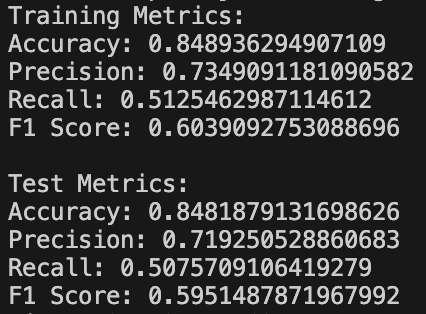
\includegraphics[width=0.5\linewidth]{GBDT_outcome.png}
    \caption*{GBDT\_Outcome}
\end{figure}
For the outcome of XGBoost:
\begin{figure}[H]
    \centering
    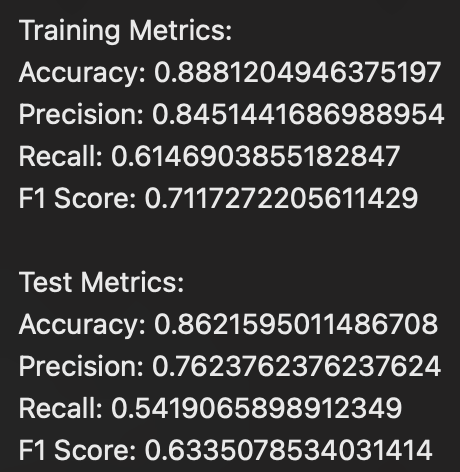
\includegraphics[width=0.5\linewidth]{XGBoost_outcome.png}
    \caption*{XGBoost\_Outcome}
\end{figure}
The improved model exhibits enhanced performance across all metrics, both on training and testing datasets. Notably, there is a substantial increase in the F1 score, which suggests a better balance between precision and recall, and this is particularly important if the model is intended for use in environments where both false positives and false negatives are to be minimized.\\

However, while the model's accuracy on the training set increased more significantly than on the test set, the difference is not drastic, which implies that overfitting is still not a significant issue. The improvements in precision and recall suggest that any issues related to class imbalance or model bias have been somewhat mitigated, although these areas could possibly still be improved.\\

From the analysis of performance above, we find that the improvement is not so huge, which is the result of a small dataset. Therefore, we also decide to compare the time of the model running.\\

For GBDT, the accurate time is $12.513447046279907$ s. And for XGBoost, the accurate time is $1.6860013008117676$ s. This improvement of the time is so huge that we cannot ignore it. XGBoost is substantially more efficient, running approximately 7.4 times faster than GBDT. As the two models both are tree-based methods, the speedup could indicate a reduction in complexity, like fewer trees or shallower trees, which can result in a faster execution time.\\

In summary, not only has the improved model's predictive performance increased, but it is also much faster, which can be highly beneficial for deployment in production environments where both accuracy and speed are critical.

\newpage

\section*{Appendix: Task Division}
\begin{itemize}
    \item \textbf{LIN YI-HSUAN (Student ID: A0275070J)} is responsible for:
    \begin{itemize}
        \item The dataset section, including dataset introduction, data preprocessing, and data visualization.
        \item The introduction and usage of the XGBoost method.
        \item Compilation of related literature.
    \end{itemize}
    
    \item \textbf{HUANG RUI (Student ID: A0275006L)} is responsible for:
    \begin{itemize}
        \item Overall task introduction.
        \item The introduction and usage of the GBDT method.
        \item Comparative analysis of the XGBoost and GBDT methods.
        \item Compilation of related literature.
    \end{itemize}
\end{itemize}q

\section*{Appendix: Code Implementation}
\subsection*{GBDT}
\begin{minted}{python}
import requests
import pandas as pd
from io import StringIO
from sklearn.model_selection import train_test_split
from sklearn.preprocessing import LabelEncoder, StandardScaler, OneHotEncoder
from sklearn.compose import ColumnTransformer
from sklearn.impute import SimpleImputer
from sklearn.pipeline import Pipeline
from sklearn.ensemble import GradientBoostingClassifier
from sklearn.metrics import accuracy_score, precision_score, recall_score, f1_score
import time


url = "https://tianchi-media.oss-cn-beijing.aliyuncs.com/DSW/7XGBoost/train.csv"
response = requests.get(url)

if response.status_code == 200:
    data = StringIO(response.text)
    df = pd.read_csv(data)
    
    numerical_cols = df.select_dtypes(include=['int64', 'float64']).columns.tolist()
    categorical_cols = df.select_dtypes(include=['object']).columns.tolist()
  
    if 'RainTomorrow' in categorical_cols:
        categorical_cols.remove('RainTomorrow')

    numeric_transformer = Pipeline(steps=[
        ('imputer', SimpleImputer(strategy='median')),
        ('scaler', StandardScaler())
    ])

    categorical_transformer = Pipeline(steps=[
        ('imputer', SimpleImputer(strategy='constant', fill_value='missing')),
        ('onehot', OneHotEncoder(handle_unknown='ignore'))
    ])

    preprocessor = ColumnTransformer(
        transformers=[
            ('num', numeric_transformer, numerical_cols),
            ('cat', categorical_transformer, categorical_cols)
        ])
    

    X = df.drop('RainTomorrow', axis=1)
    y = LabelEncoder().fit_transform(df['RainTomorrow'].astype(str))
    X_processed = preprocessor.fit_transform(X)
    
    #Split data into training and test sets
    X_train, X_test, y_train, y_test = train_test_split(X_processed, y,
        test_size=0.2, random_state=42)
    #print(df.head())
else:
    print("Failed to load data")

start_time = time.time()
clf = GradientBoostingClassifier(n_estimators=100,learning_rate=1.0,max_depth=1,
    random_state=0)
clf = clf.fit(X_train, y_train)
predictions_train = clf.predict(X_train)
predictions_test = clf.predict(X_test)


# accuracy
accuracy_train = accuracy_score(y_train, predictions_train)
accuracy_test = accuracy_score(y_test, predictions_test)

# precision
precision_train = precision_score(y_train, predictions_train, average='binary')
precision_test = precision_score(y_test, predictions_test, average='binary')

# recall
recall_train = recall_score(y_train, predictions_train, average='binary')
recall_test = recall_score(y_test, predictions_test, average='binary')

# F1 score
f1_train = f1_score(y_train, predictions_train, average='binary')
f1_test = f1_score(y_test, predictions_test, average='binary')

print("Training Metrics:")
print(f"Accuracy: {accuracy_train}")
print(f"Precision: {precision_train}")
print(f"Recall: {recall_train}")
print(f"F1 Score: {f1_train}")

print("\nTest Metrics:")
print(f"Accuracy: {accuracy_test}")
print(f"Precision: {precision_test}")
print(f"Recall: {recall_test}")
print(f"F1 Score: {f1_test}")
end_time = time.time()
print('Time:', end_time - start_time)
\end{minted}
\subsection*{XGBoost}
\begin{minted}{python}
import numpy as np 
import pandas as pd
import matplotlib.pyplot as plt
import seaborn as sns
from xgboost.sklearn import XGBClassifier
from sklearn import metrics
from sklearn.preprocessing import LabelEncoder

import requests
from io import StringIO
from sklearn.model_selection import train_test_split
from sklearn.preprocessing import LabelEncoder, StandardScaler, OneHotEncoder
from sklearn.compose import ColumnTransformer
from sklearn.impute import SimpleImputer
from sklearn.pipeline import Pipeline
import matplotlib.pyplot as plt
import seaborn as sns

url = "https://tianchi-media.oss-cn-beijing.aliyuncs.com/DSW/7XGBoost/train.csv"
response = requests.get(url)

if response.status_code == 200:
    data = StringIO(response.text)
    df = pd.read_csv(data)
    
    numerical_cols = df.select_dtypes(include=['int64', 'float64']).columns.tolist()
    categorical_cols = df.select_dtypes(include=['object']).columns.tolist()
  
    if 'RainTomorrow' in categorical_cols:
        categorical_cols.remove('RainTomorrow')

    numeric_transformer = Pipeline(steps=[
        ('imputer', SimpleImputer(strategy='median')),
        ('scaler', StandardScaler())
    ])

    categorical_transformer = Pipeline(steps=[
        ('imputer', SimpleImputer(strategy='constant', fill_value='missing')),
        ('onehot', OneHotEncoder(handle_unknown='ignore'))
    ])

    preprocessor = ColumnTransformer(
        transformers=[
            ('num', numeric_transformer, numerical_cols),
            ('cat', categorical_transformer, categorical_cols)
        ])
    
X = df.drop('RainTomorrow', axis=1)
y = LabelEncoder().fit_transform(df['RainTomorrow'].astype(str))

# Using ColumnTransformer for preprocessing
preprocessor = ColumnTransformer(
    transformers=[
        ('num', numeric_transformer, numerical_cols), 
        # Apply transformations to numerical columns
        ('cat', categorical_transformer, categorical_cols)  
        # Apply transformations to categorical columns
    ])

# Apply preprocessing transformation
X_processed = preprocessor.fit_transform(X)

# Split the data into training and testing sets
X_train, X_test, y_train, y_test = train_test_split(X_processed, y, test_size=0.2, 
random_state=42)

# Here we define X_train_processed and X_test_processed
X_train_processed = X_train
X_test_processed = X_test

# Data visualization
# 1. Scatter plot visualization of three features with label combinations
sns.pairplot(data=df[['Rainfall', 'Evaporation', 'Sunshine', 'RainTomorrow']],
diag_kind='hist', hue= 'RainTomorrow')
plt.show()

# 2. Bar plot visualization based on categorical features
categorical_cols = df.select_dtypes(include=['object']).columns.tolist()
if 'RainTomorrow' in categorical_cols:
    categorical_cols.remove('RainTomorrow')

# Count the values of categorical features for labels "Yes" and "No"
tlog = {}
flog = {}
for i in categorical_cols:
    tlog[i] = df[df['RainTomorrow'] == 'Yes'][i].value_counts()
    flog[i] = df[df['RainTomorrow'] == 'No'][i].value_counts()

# Take 'Location' as an example and draw bar plots
plt.figure(figsize=(10,10))
plt.subplot(1,2,1)
plt.title('RainTomorrow')
sns.barplot(x = pd.DataFrame(tlog['Location']).sort_index()['Location'], 
y = pd.DataFrame(tlog['Location']).sort_index().index, color = "red")
plt.subplot(1,2,2)
plt.title('Not RainTomorrow')
sns.barplot(x = pd.DataFrame(flog['Location']).sort_index()['Location'], 
y = pd.DataFrame(flog['Location']).sort_index().index, color = "blue")
plt.show()

# 3.Calculate the correlation matrix among numerical features and 'RainTomorrow'
# Ensure 'RainTomorrow' is of a numerical type, if not, convert it
if df['RainTomorrow'].dtype == object:
    from sklearn.preprocessing import LabelEncoder
    le = LabelEncoder()
    df['RainTomorrow'] = le.fit_transform(df['RainTomorrow'])

# Select numerical columns from df
numerical_features = df.select_dtypes(include=['int64', 'float64']).columns.tolist()

# If 'RainTomorrow' is not in the list of numerical features, add it
if 'RainTomorrow' not in numerical_features:
    numerical_features.append('RainTomorrow')

# Calculate the correlation matrix
corr_matrix = df[numerical_features].corr()

# Draw the heatmap
plt.figure(figsize=(12, 8))
sns.heatmap(corr_matrix, annot=True, cmap='coolwarm', fmt=".2f")
plt.title('Correlation Heatmap Between Features and RainTomorrow')
plt.show()

# 4. Filter the data for 'RainTomorrow' equals 'Yes' and 'No'
rain_yes = df[df['RainTomorrow'] == 1]['Rainfall'].dropna()
rain_no = df[df['RainTomorrow'] == 0]['Rainfall'].dropna()

# Function to calculate the Cumulative Distribution Function (CDF)
def calc_cdf(data):
    n = len(data)
    x = np.sort(data)  # sort data in ascending order
    y = np.arange(1, n+1) / n  # calculate the cumulative percentage
    return x, y

x_yes, y_yes = calc_cdf(rain_yes)
x_no, y_no = calc_cdf(rain_no)

# Plotting the CDF for rainfall where 'RainTomorrow' is 'Yes' and 'No'
plt.figure(figsize=(10, 6))
plt.plot(x_yes, y_yes, label='RainTomorrow = Yes', marker='.', linestyle='none')
plt.plot(x_no, y_no, label='RainTomorrow = No', marker='.', linestyle='none')
plt.legend()
plt.xlabel('Rainfall')
plt.ylabel('CDF')
plt.title('CDF of Rainfall by RainTomorrow')
plt.margins(0.02)  # Ensures a bit of margin on the sides of the plot
plt.show()


import time
start_time = time.time()
# Train the XGBoost model and adjust model parameters
model = XGBClassifier(
    use_label_encoder=False, 
    eval_metric='logloss', 
    n_estimators=200,  # Increase the number of trees
    max_depth=8,       # Increase the depth of trees
    learning_rate=0.1  # Adjust the learning rate
)
model.fit(X_train_processed, y_train)  # Ensure using preprocessed data

# Predictions
predictions_train = model.predict(X_train_processed)
predictions_test = model.predict(X_test_processed)

# Evaluation
print('Training Accuracy:', metrics.accuracy_score(y_train, predictions_train))
print('Test Accuracy:', metrics.accuracy_score(y_test, predictions_test))
end_time = time.time()
print("time:", end_time - start_time, "seconds")
# Feature importance visualization
plt.figure(figsize=(10, 8))
sns.barplot(y=np.arange(len(model.feature_importances_)), x=model.feature_importances_)
plt.title('Feature Importances')
plt.xlabel('Importance')
plt.ylabel('Feature indices')
plt.show()

from sklearn.metrics import accuracy_score, precision_score, recall_score, f1_score

# accuracy
accuracy_train = accuracy_score(y_train, predictions_train)
accuracy_test = accuracy_score(y_test, predictions_test)

# precision
precision_train = precision_score(y_train, predictions_train, average='binary')
precision_test = precision_score(y_test, predictions_test, average='binary')

# recall
recall_train = recall_score(y_train, predictions_train, average='binary')
recall_test = recall_score(y_test, predictions_test, average='binary')

# F1 score
f1_train = f1_score(y_train, predictions_train, average='binary')
f1_test = f1_score(y_test, predictions_test, average='binary')

print("Training Metrics:")
print(f"Accuracy: {accuracy_train}")
print(f"Precision: {precision_train}")
print(f"Recall: {recall_train}")
print(f"F1 Score: {f1_train}")

print("\nTest Metrics:")
print(f"Accuracy: {accuracy_test}")
print(f"Precision: {precision_test}")
print(f"Recall: {recall_test}")
print(f"F1 Score: {f1_test}")

\end{minted}


\begin{thebibliography}{99}

\bibitem{friedman2001greedy} 
Friedman, J. H. (2001). \textit{Greedy function approximation: A gradient boosting machine}. The Annals of Statistics, 29(5), 1189–1232. \url{https://doi.org/10.1214/aos/1013203451}
\bibitem{chen2016xgboost}
Chen, T., \& Guestrin, C. (2016). \textit{XGBoost: A Scalable Tree Boosting System}. In \textit{22nd SIGKDD Conference on Knowledge Discovery and Data Mining}.







\end{thebibliography}






\end{document}